\documentclass[10pt]{article}

\usepackage{graphicx}
\usepackage{amsmath,amsfonts,amssymb}

% use different colors for links:
\usepackage{color}
\definecolor{darkgreen}{rgb}{0.1,0.5,0.1}
\definecolor{darkblue}{rgb}{0.2,0.2,1.0}
\usepackage[colorlinks=true,linkcolor=darkblue,citecolor=darkblue,
            filecolor=darkblue,urlcolor=darkgreen]{hyperref}


\setlength{\textwidth}{6.2in}
\setlength{\oddsidemargin}{0.3in}
\setlength{\evensidemargin}{0in}
\setlength{\textheight}{8.9in}
\setlength{\voffset}{-1in}
\setlength{\headsep}{26pt}
\setlength{\parindent}{0pt}
\setlength{\parskip}{5pt}




% a few handy macros

\newcommand\matlab{{\sc matlab}}
\newcommand{\goto}{\rightarrow}
\newcommand{\bigo}{{\mathcal O}}
\newcommand{\half}{\frac{1}{2}}
%\newcommand\implies{\quad\Longrightarrow\quad}
\newcommand\reals{{{\rm l} \kern -.15em {\rm R} }}
\newcommand\complex{{\raisebox{.043ex}{\rule{0.07em}{1.56ex}} \hskip -.35em {\rm C}}}


% macros for matrices/vectors:

% matrix environment for vectors or matrices where elements are centered
\newenvironment{mat}{\left[\begin{array}{ccccccccccccccc}}{\end{array}\right]}
\newcommand\bcm{\begin{mat}}
\newcommand\ecm{\end{mat}}

% matrix environment for vectors or matrices where elements are right justifvied
\newenvironment{rmat}{\left[\begin{array}{rrrrrrrrrrrrr}}{\end{array}\right]}
\newcommand\brm{\begin{rmat}}
\newcommand\erm{\end{rmat}}

% for left brace and a set of choices
\newenvironment{choices}{\left\{ \begin{array}{ll}}{\end{array}\right.}
\newcommand\when{&\text{if~}}
\newcommand\otherwise{&\text{otherwise}}
% sample usage:
%  \delta_{ij} = \begin{choices} 1 \when i=j, \\ 0 \otherwise \end{choices}


% for labeling and referencing equations:
\newcommand{\eql}{\begin{equation}\label}
\newcommand{\eqn}[1]{(\ref{#1})}
% can then do
%  \eql{eqnlabel}
%  ...
%  \end{equation}
% and refer to it as equation \eqn{eqnlabel}.  


% some useful macros for finite difference methods:
\newcommand\unp{U^{n+1}}
\newcommand\unm{U^{n-1}}

% for chemical reactions:
\newcommand{\react}[1]{\stackrel{K_{#1}}{\rightarrow}}
\newcommand{\reactb}[2]{\stackrel{K_{#1}}{~\stackrel{\rightleftharpoons}
   {\scriptstyle K_{#2}}}~}

% Parts:

% set enumerate to give parts a, b, c, ...  rather than numbers 1, 2, 3...
\renewcommand{\theenumi}{\alph{enumi}}
\renewcommand{\labelenumi}{(\theenumi)}

% set second level enumerate to give parts i, ii, iii, iv, etc.
\renewcommand{\theenumii}{\roman{enumii}}
\renewcommand{\labelenumii}{(\theenumii)}

  % input some useful macros

\begin{document}

% header:
\hfill\vbox{\hbox{AMath 586 / ATM 581}
\hbox{Homework \#3}\hbox{Due Thursday, April 30, 2015}}

\vskip 5pt

Homework is due to Canvas by 11:00pm PDT on the due date.

To submit, see \url{https://canvas.uw.edu/courses/962872/assignments/}


%--------------------------------------------------------------------------
\vskip 1cm
\hrule
{\bf Problem 1}  


Let $g(x)=0$ represent a system of $s$ nonlinear equations in $s$ unknowns,
so $x\in\reals^s$ and $g: \reals^s \goto \reals^s$.  A vector $\bar
x\in\reals^s$ is a {\em fixed point} of $g(x)$ if 
\begin{equation}\label{a}
\bar x = g(\bar x).
\end{equation}
One way to attempt to compute $\bar x$ is with {\em fixed point iteration}:
from some starting guess $x^0$, compute
\begin{equation}\label{b}
x^{j+1} = g(x^j)
\end{equation}
for $j=0,~1,~\ldots$.

\begin{enumerate}
\item Show that if there exists a norm $\|\cdot\|$ such that $g(x)$ is
Lipschitz continuous with constant $L<1$ in a neighborhood of $\bar x$, then
fixed point iteration converges from any starting value in this
neighborhood.
{\bf Hint:} Subtract equation \eqn{a} from \eqn{b}.

\item Suppose $g(x)$ is differentiable and let $g'(x)$ be the $s\times s$
Jacobian matrix.  Show that if the condition of part (a) holds then
$\rho(g'(\bar x)) < 1$, where $\rho(A)$ denotes the spectral radius of a
matrix.

\item Consider a predictor-corrector method (see Section 5.9.4) consisting
of forward Euler as the predictor and backward Euler as the corrector, and
suppose we make $N$ correction iterations, i.e., we set
\begin{tabbing}
xxxxxxxxx\=xxxx\=\kill\\
\>$\hat U^0 = U^n + kf(U^n)$\\
\>for $j = 0,~1,~\ldots,~N-1$\\
\>\>$\hat U^{j+1} = U^n + kf(\hat U^j)$\\
\>\>end\\
\>$U^{n+1} = \hat U^N$.
\end{tabbing}
Note that this can be interpreted as a fixed point iteration for solving the
nonlinear equation
\[
\unp = U^n + kf(\unp)
\]
of the backward Euler method.  Since the backward Euler method is implicit
and has a stability region that includes the entire left half plane, as
shown in Figure 7.1(b), one might hope that this predictor-corrector method
also has a large stability region.

Plot the stability region $S_N$
of this method for $N=2,~5,~10,~20$ (perhaps using
{\tt plotS.m} from the webpage) and observe that in fact the stability
region does not grow much in size.

\item Using the result of part (b), show that the fixed point iteration
being used in the predictor-corrector method of part (c) can only be
expected to converge if $|k\lambda| < 1$ for all eigenvalues $\lambda$ of the
Jacobian matrix $f'(u)$.  

\item Based on the result of part (d) and the shape of the stability region
of Backward Euler, what do you expect the stability region $S_N$ of part (c)
to converge to as $N\goto\infty$?

\end{enumerate}




% uncomment the next two lines if you want to insert solution...
%\vskip 1cm
%{\bf Solution:}

% insert your solution here!

%--------------------------------------------------------------------------
\newpage
\vskip 1cm
\hrule
{\bf Problem 2}  

Use the Boundary Locus method to plot the stability region for the TR-BDF2
method (8.6).   You can use the Matlab script \texttt{makeplotS.m}
from the book website, or a Python script as illustrated in 
{\tt \$AM586/codes/notebook3.ipynb}
(To view online, see 
\url{http://faculty.washington.edu/rjl/classes/am586s2015/codes.html})

Observe that the method is A-stable and show that it is
also L-stable.


% uncomment the next two lines if you want to insert solution...
%\vskip 1cm
%{\bf Solution:}

% insert your solution here!

%--------------------------------------------------------------------------
\vskip 1cm
\hrule
{\bf Problem 3}  

The goal of this problem is to write a very simple adaptive time step ODE
solver based on the Bogacki--Shampine Runge--Kutta method.  This is a
third-order accurate 4-stage method that also produces a second-order
accurate approximation each time step that can be used for error estimation. 
(This is the method used in the Matlab routine \texttt{ode23}.)

See, e.g. \url{http://en.wikipedia.org/wiki/Bogacki-Shampine\_method}
for a description and the coefficients. 

Note that it appears to require 4 evaluations of $f$ each time step, but the
last one needed in one step can be re-used in the next step.  You should
take advantage of this to reduce it to 3 new $f$-evaluations each step.

In lecture, I discussed the method (5.42) in which $U^{n+1}$ is used for the
next time step and is second-order accurate, while $\hat U^{n+1}$ is 
``first-order accurate'', which means the 1-step error is $\bigo(k^2)$, and
this is what is approximated by the difference $|U^{n+1}-\hat U^{n+1}|$.

For the Bogacki--Shampine method, the corresponding difference $|U^{n+1}-\hat
U^{n+1}|$ will be approximately equal to the 1-step error of the second order
method, so we expect it to have the form $k_n\tau^n \approx C_n k_n^3$, where
$k_n$ is the time
step just used in the $n$th step, and $C_n$ is a constant that will depend
on how smooth the solution is near time $t_n$.  After each time step, we
can estimate this by
\begin{equation}\label{Cn}
C_n \approx |U^{n+1}-\hat U^{n+1}|^{1/3}.
\end{equation} 
If we were simply using the second order method and trying to achieve an
absolute error less than some $\epsilon$ over the time interval $t_0 \leq t
\leq T$, then we would want to choose our time steps so that 
\[
|\tau^n| \leq \epsilon / (T-t_0)
\]
Then if we assume the method is behaving stably and we estimate the global
error at time $T$ by the sum of the one-step errors, this is roughly
\[
\sum_m k_m |\tau^m| \leq \left(\sum k_m\right) \frac{\epsilon}{T-t_0} =
\epsilon.
\]
Convince yourself that this suggests choosing the next time step as
\begin{equation}\label{kn}
\left(\frac{\epsilon}{C_n(T-t_0)}\right)^{1/2}.
\end{equation} 

Note that we have already taken a step with time step $k_n$ in order to
approximate $C_n$, so the simplest approach is just to use \eqn{kn}
to define our {\em next} time step $k_{n+1}$, with $C_n$ estimated
from \eqn{Cn}.  (A more sophisticated method would go back and
re-take a smaller step if the estimate indicates we took a step
that was too large.)

Note that the error estimate is based on the second-order method, but the
value we take for our next step is $U^{n+1}$, which we hope is even more
accurate.

\newpage
Implement this idea, with the following steps:

\begin{itemize} 
\item First implement a function that takes a single time step with the B--S
method and confirm that it is working, e.g. if you apply it to $u' = -u$
for a single step of size $k$ the errors behave as expected when you reduce
$k$.  

\item Then implement a fixed time step method based on this and verify that
the method is third-order accurate.

\item Implement an adaptive time version and test it on various 
problems where you know the solution.

\end{itemize} 

{\bf Note:} You will need to choose a time step for the first step.  To keep
it simple, just use $k_0 = 10^{-4}$.   You should also set some maximum
step size that's allowed since there may be times when the error estimate
happens to be very small.  Take this to be $k_{max} = 10 \epsilon^{1/3}$.

{\bf Note:} Do not expect this method to work all that well.  The main point
is to get some idea of how adaptive time stepping works and some of the
issues that make it difficult to write a general purpose code of this
nature.  There is software available that does a very good job (e.g. in
Matlab or SciPy, and the codes these are built on), but a lot of
work has gone into tuning these.


Once your code is working, try it on problems of the form

\begin{equation}\label{fuv}
u'(t) = \lambda (u - v(t)) + v'(t)
\end{equation} 
where $v(t)$ is a desired exact solution and the initial data is chosen as 
$u(0) = v(0)$.

In particular, try the following.  Produce some sample plots of the
solutions and also plots of the error and step size used as functions of
$t$, as illustrated in the figures below.

\begin{enumerate} 
\item  Exact solution
\[
v(t) = \cos(t) 
\]
for $0\leq t \leq 10$ and $\lambda = -1$. Try different tolerances
$\epsilon$ in the range $10^{-2}$ to $10^{-10}$.

\item
Try the above problem with more negative $\lambda$, e.g. $\lambda=-100$.
What happens if $\epsilon$ is large enough that $k_{acc} > k_{stab}$?  Does
the method go unstable?


\item  Exact solution
\[
v(t) = \cos(t) + \exp\left(-80(t-2)^2\right),
\]
for $0\leq t \leq 4$ and $\lambda = -1$. The Gaussian gives a region where the
solution is much more rapidly varying and smaller time steps are required. 

You might get something as shown in the figure below
(obtained from my code with $\epsilon = 10^{-2}$).   
But the results are quite sensitive to small changes in the algorithm, so
don't expect to match this exactly!

\vskip 5pt
\hfil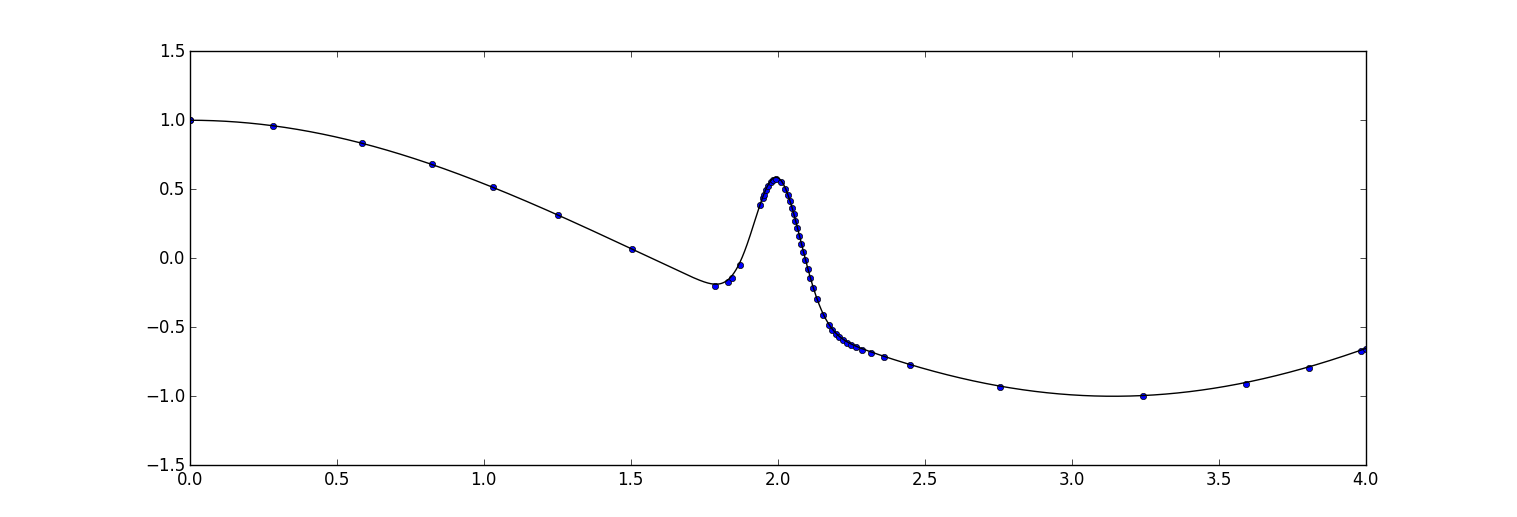
\includegraphics[width=5.5in]{u.png}\hfil
\vskip 5pt
\hfil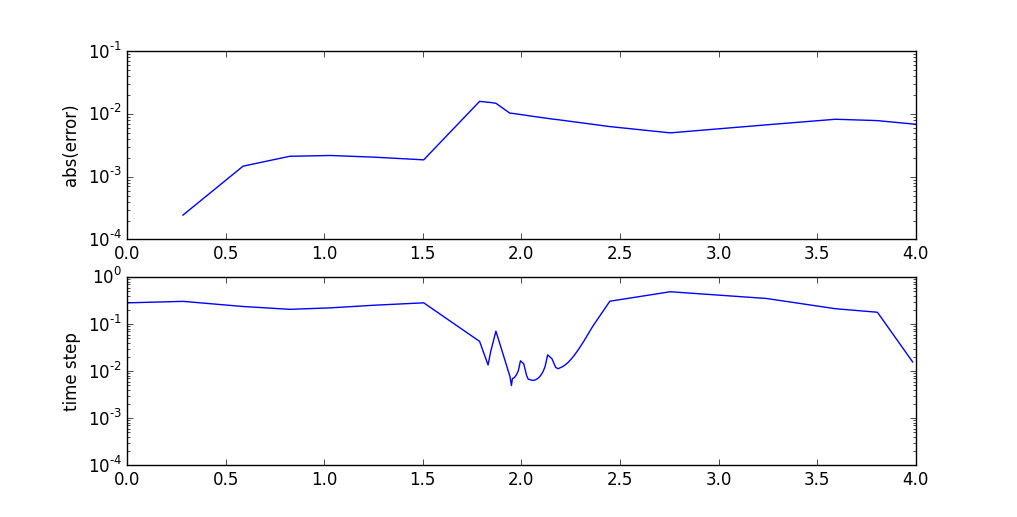
\includegraphics[width=5.5in]{errdt.png}\hfil
\vskip 5pt



\end{enumerate} 



% uncomment the next two lines if you want to insert solution...
%\vskip 1cm
%{\bf Solution:}

% insert your solution here!

%--------------------------------------------------------------------------

\end{document}

